\documentclass[tikz,border=10pt]{standalone}
\usepackage{tikz}
\usetikzlibrary{calc}

\begin{document}
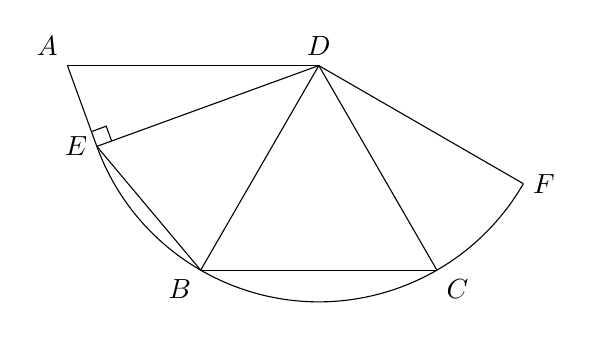
\begin{tikzpicture}
    % Define coordinates
    \coordinate (D) at (0, 0);
    \def\R{3}
    
    % Angles for points on the circle
    % E at 200 degrees
    % B at 240 degrees
    % C at 300 degrees (symmetric to B for horizontal BC)
    % F at 330 degrees
    
    \coordinate (E) at ({\R * cos(200)}, {\R * sin(200)});
    \coordinate (B) at ({\R * cos(240)}, {\R * sin(240)});
    \coordinate (C) at ({\R * cos(300)}, {\R * sin(300)});
    \coordinate (F) at ({\R * cos(330)}, {\R * sin(330)});
    
    % Calculate A: intersection of tangent at E and y=0 (to the left)
    % Tangent direction at E (200 deg) is 110 deg or 290 deg.
    % We want to go up to y=0, so 110 deg.
    % Line: E + t * (cos 110, sin 110)
    % y = y_E + t * sin 110 = 0 => t = -y_E / sin 110
    \pgfmathsetmacro{\yE}{\R * sin(200)}
    \pgfmathsetmacro{\xE}{\R * cos(200)}
    \pgfmathsetmacro{\t}{-\yE / sin(110)}
    \pgfmathsetmacro{\xA}{\xE + \t * cos(110)}
    \coordinate (A) at (\xA, 0);
    
    % Draw Arc E-B-C-F
    \draw (E) arc (200:330:\R);
    
    % Draw Chords EB and BC
    \draw (E) -- (B);
    \draw (B) -- (C);
    
    % Draw Radii
    \draw (D) -- (E);
    \draw (D) -- (B);
    \draw (D) -- (C);
    \draw (D) -- (F);
    
    % Draw Line AD
    \draw (A) -- (D);
    
    % Draw Line AE
    \draw (A) -- (E);
    
    % Draw Right Angle at E (between AE and DE)
    % Vector ED is D - E. Vector EA is A - E.
    % We draw a small square.
    \coordinate (E_right) at ($(E)!0.3cm!(D)$);
    \coordinate (E_up) at ($(E)!0.3cm!(A)$);
    % We need to project to make a square. 
    % Since AE is tangent and DE is radius, they are perpendicular.
    % So we can just draw lines parallel to DE and AE.
    \draw ($(E)!0.2cm!(D)$) -- ($(E)!0.2cm!(D) + ($(E)!0.2cm!(A)$) - (E)$) -- ($(E)!0.2cm!(A)$);
    
    % Labels
    \node[above left] at (A) {$A$};
    \node[below left] at (B) {$B$};
    \node[below right] at (C) {$C$};
    \node[above] at (D) {$D$};
    \node[left] at (E) {$E$};
    \node[right] at (F) {$F$};
    
\end{tikzpicture}
\end{document}
